% !TeX program = pdflatex
\documentclass[russian,utf8,emptystyle,reduceheight=5mm]{eskdtext}

% packages
%
% Тестовое наполнение текстом
% При написании работы - удалить пакет и комманды \lipsum
\usepackage{lipsum}
%
\usepackage{eskdplain}
\usepackage{graphicx}
\usepackage{datetime}
\usepackage{enumitem} % for lists
\usepackage{ulem} % for underlining
\usepackage{lastpage} % Number of pages
\usepackage{hyperref} % Links in pdf

% setup
\newcommand{\FrontPageDepartment}{ЭМ} %Факультет
\newcommand{\FrontPageSubdepartment}{Менеджмента} %Кафедра
\newcommand{\WorkType}{Контрольная работа} %Тип работы (заголовок)
\newcommand{\Subject}{Предмет} %по ... родительный падеж
\newcommand{\Topic}{Тема контрольной работы} %Тема
\newcommand{\Professor}{Иванов~И.~И.} %Руководитель
\newcommand{\Student}{Петров~П.~П.} %Студент
\newcommand{\Group}{ИСм-112} %Группа
\newcommand{\FrontPageDate}{\ddmmyyyydate\today} %Дата

\ESKDsignature{МИВУ 230400.68 ПЗ} % Код специальности и тип работы

% eskdx setup
\ESKDletter{}{У}{}
\ESKDtitle{\Topic}
\ESKDchecker{\Professor}
\ESKDauthor{\Student}
\ESKDcolumnIX{МИ ВлГУ\\ \Group}

\addto\captionsrussian{\def\refname{Список использованных источников}}
\sloppy % split long lines

% graphics path
\graphicspath{{src/img/}}


% verbatim setup
\newcommand{\verbatimFont}{
\fontsize{10pt}{12pt}\selectfont
\baselineskip=1em
}


% workaround for regression in babel package on linux
\providecommand{\No}{\textnumero}


% remove vertical space from lists
%\renewcommand{\alph}[1]{\asbuk{#1}} % костыль для кирилической нумерации вместо латинской
\setlist{nolistsep} % убираем дополнительные вертикальные отступы вокруг списков
\setenumerate[1]{label=\arabic*), fullwidth, itemindent=\parindent,  listparindent=\parindent}
\setenumerate[2]{label=\arabic*), fullwidth, itemindent=\parindent, listparindent=\parindent, leftmargin=\parindent}
\setitemize{fullwidth, itemindent=\parindent, listparindent=\parindent}
\newlength{\PAGEborderLR}
\newlength{\PAGEborderTB}

\setlength{\PAGEborderLR}{2cm}
\setlength{\PAGEborderTB}{2cm}

% Set up page
\setlength{\hoffset}{-2.54cm + \PAGEborderLR}
\setlength{\voffset}{-2.54cm + \PAGEborderTB}
\setlength{\topskip}{0pt}
\setlength{\footskip}{21pt}
\setlength{\oddsidemargin}{0pt}
\setlength{\evensidemargin}{0pt}
\setlength{\topmargin}{0pt}
\setlength{\headheight}{0pt}
\setlength{\headsep}{0pt}
\setlength{\textwidth}{210mm-\PAGEborderLR*2}
\setlength{\textheight}{297mm-\PAGEborderTB*2-\footskip}
\setlength{\marginparsep}{0pt}
\setlength{\marginparwidth}{0pt}
\setlength{\marginparpush}{0pt}

% main document
\begin{document}
% Титул
\ESKDthisStyle{empty}
\setlength{\topskip}{15pt}
\newlength{\frontpagefk} % Ширина поля Факультет/Кафедра
\setlength{\frontpagefk}{6cm}
\newlength{\frontpagerb} % Ширина надписей Руководитель/Студент и пр. под темой
\setlength{\frontpagerb}{6cm}
\newlength{\frontpagerbspace} % ??? (do not remove)
\setlength{\frontpagerbspace}{1cm}
\newlength{\FrontPageSubjSpace} % Ширина пробела до и после названия предмета
\setlength{\FrontPageSubjSpace}{1cm}
\newlength{\FrontPageTopicSpace} % Ширина пробела до и после темы
\setlength{\FrontPageTopicSpace}{0.5cm}

\thispagestyle{empty}
\begin{center}
{
\vspace*{-1.5cm}
\baselineskip=1.3em
{\small Министерство образования и науки Российской Федерации}\\
\textbf{Муромский институт (филиал)}\\
{\footnotesize федерального государственного бюджетного образовательного учреждения\\
высшего профессионального образования}\\
\textbf{<<Владимирский государственный университет\\
имени Александра Григорьевича и Николая Григорьевича\\
Столетовых>>\\
(МИ (филиал) ВлГУ)\\}
}

\bigskip
\begin{tabular}{l c}
\textbf{Факультет}&\underline{\makebox[\frontpagefk]{\FrontPageDepartment}}\\
\textbf{Кафедра}&\underline{\makebox[\frontpagefk]{\FrontPageSubdepartment}}\\
\end{tabular}

\vspace{\fill}
\begin{Huge}
\textsl{\WorkType}
\end{Huge}

\vspace{\fill}
по \underline{\makebox[\FrontPageSubjSpace]{}\Subject\makebox[\FrontPageSubjSpace]{}}

\smallskip
\parbox{15cm}{\centering{Тема: \uline{\makebox[\FrontPageTopicSpace]{}\Topic\makebox[\FrontPageTopicSpace]{}}}}

\vspace{\fill}

\begin{flushright}
\makebox[\frontpagerb][c]{
\makebox[\frontpagerb][l]{Руководитель}\hspace{\frontpagerbspace}}

\smallskip
\makebox[\frontpagerb][c]{
\raisebox{-\baselineskip}{\shortstack{\underline{\makebox[\frontpagerb][l]{\Professor}}\\
\begin{footnotesize}
(фамилия, инициалы)
\end{footnotesize}}}\hspace{\frontpagerbspace}}

\bigskip
\makebox[\frontpagerb][c]{
\raisebox{-\baselineskip}{\shortstack{\underline{\makebox[\frontpagerb][l]{}}\\
\begin{footnotesize}
(подпись)\hfill(дата)
\end{footnotesize}}}\hspace{\frontpagerbspace}}

\newcommand{\frontpagerbstudent}[2]{ %
\makebox[\frontpagerb]{ %
\raisebox{-\baselineskip}{\shortstack{#1\ \underline{\makebox[\frontpagerb-\widthof{#1\ }][c]{#2}}\\
\begin{footnotesize}
\makebox[\widthof{#1\ }][c]{}\makebox[\frontpagerb-\widthof{#1\ }][c]{(группа)}
\end{footnotesize}}}\hspace{\frontpagerbspace}}
}

\bigskip
\makebox[\frontpagerb][c]{\frontpagerbstudent{Студент}{\Group}}

\smallskip
\makebox[\frontpagerb][c]{
\raisebox{-\baselineskip}{\shortstack{\underline{\makebox[\frontpagerb][l]{\Student}}\\
\begin{footnotesize}
(фамилия, инициалы)
\end{footnotesize}}}\hspace{\frontpagerbspace}}

\renewcommand{\dateseparator}{.}

\bigskip
\makebox[\frontpagerb][c]{
\raisebox{-\baselineskip}{\shortstack{\underline{\makebox[\frontpagerb][r]{\FrontPageDate}}\\
\begin{footnotesize}
(подпись)\hfill(дата)
\end{footnotesize}}}\hspace{\frontpagerbspace}}

\end{flushright}

\vspace{\fill}
Муром -- \the\year
\vspace*{-1cm}
\end{center}
\setlength{\topskip}{0pt}
\newpage

% Аннотация
\ESKDthisStyle{empty}
\vspace*{\fill}
Курсовой проект посвящен разработке и реализации ...

В курсовом проекте подробно описано техническое задание, проведена разработка алгоритмов, программы, написано руководство, осуществлено тестирование системы.

Объём пояснительной записки составляет \pageref{LastPage} листов. Количество рисунков - 2 штуки. Таблицы отсутствуют.
\vspace*{\fill}
\newpage

% Содержание
\setcounter{page}{4}
\tableofcontents
\newpage

% Основной текст
\begin{center}
\textbf{Лабораторная работа №5}
\\
\textbf Работа с пакетным менеджером для С++
\\
\end{center}
\textbf{Порядок выполнения:} 
\begin{enumerate}
\item Запустить VS.
\item Создать проект С++ -> CMake. При создание проекта снять флажок “Создать папку для проекта”.
\item Выполнить сборку созданного проекта
\item Открыть главный CMakeLists.txt (в самой верхней папке)
\item До строки add\_executable добавить
find\_package(CPPAN REQUIRED)
cppan\_add\_package(
	pvt.cppan.demo.intel.opencv.highgui-3
)
cppan\_execute()
\item После строки
 add\_executable добавить
target\_link\_libraries
(ПервыйАргументИзAddExecutable
	pvt.cppan.demo.intel.opencv.highgui
)
\item В файле с кодом (.cpp файл) подключить заголовочный файл
#include <opencv2/highgui.hpp>
\item В функцию main() добавить код для открытия изображения в формате png и сохранения файла в формате bmp.

 
\\
\end{enumerate}
\newpage
CMakeProject1.cpp:\\
// CMakeProject1.cpp: определяет точку входа для приложения.\\
//
\#include <opencv2/highgui.hpp>\\
\#include "CMakeProject1.h"\\

using namespace std;\\

int main()\\
{
	cout << "Hello CMake." << endl\\
	auto i = cv::imread("E:\\student\\picta.png");\\
	i = 255 - i; // инверсия изображения\\
	cv::imwrite("E:\\student\\img.bmp", i);
\\
	return 0;\\
}



\newpage
CMakeList.txt:\\

\# CMakeList.txt: проект CMake для CMakeProject1; включите исходный код и определения
\# укажите здесь логику для конкретного проекта.
\#
cmake\_minimum\_required (VERSION 3.8)

find\_package(CPPAN REQUIRED)
cppan\_add\_package(
	pvt.cppan.demo.intel.opencv.highgui-3
)
cppan\_execute()

\# Добавьте источник для исполняемого файла этого проекта.
add\_executable (CMakeProject1 "CMakeProject1.cpp" "CMakeProject1.h")

\# TODO: Добавьте тесты и целевые объекты, если это необходимо.
			
target\_link\_libraries(CMakeProject1 pvt.cppan.demo.intel.opencv.highgui)


\begin{figure}[h]
\centering
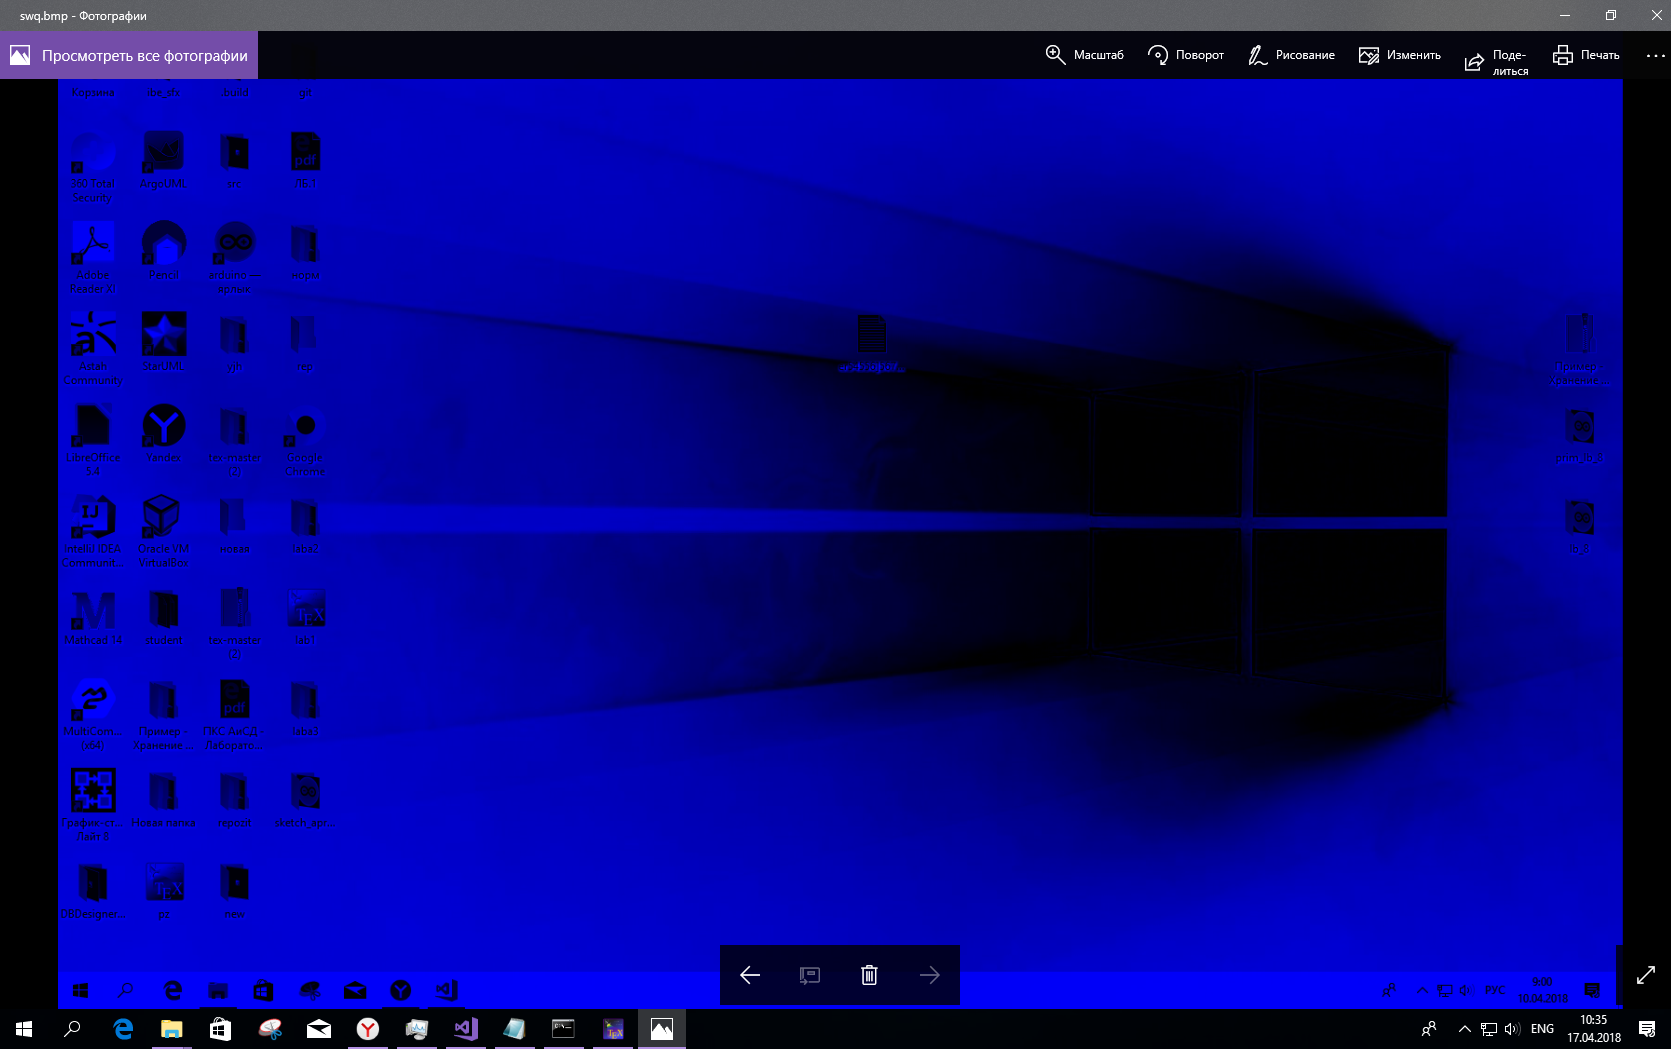
\includegraphics[scale=0.4]{ght}
\caption{Результат}
\label{fig:ght}
\end{figure}


\textbf{Вывод:} Я научился работать с пакетами для с++;




\newpage

% Список литературы
\input{src/bibliography.tex}
\end{document}